% !TEX TS-program = pdflatexmk
%\InputIfFileExists{a4-mancs.sty}{}{}

\documentclass[12pt,BSc,wordcount,twoside, openany, oneside]{muthesis}
\usepackage[a4paper, total={6.5in, 8in}]{geometry}
\usepackage{csquotes}

\usepackage{titlesec}
\titleformat{\chapter}[display]{\normalfont\bfseries}{}{0pt}{\Huge}

%\let\subparagraph\paragraph
%\let\paragraph\subsubsection
\let\subsubsection\subsection
\let\subsection\section
\let\section\chapter

%\let\chaptername\relax


%% Any characters from a % to the end of line are comments.

%% The third-rep class and this starter kit were written by 
%% Graham Gough <graham@cs.man.ac.uk>
%% If you have any comments or questions regarding this document,
%% please post them to the local newsgroup man.cs.tex.

%% This skeleton report is organised as a master file called
%% report.tex which then includes files for individual parts including
%% abstract.tex, chapter1.tex, chapter2.tex, chapter3.tex and
%% appendix1.tex.  

%% The third-rep style is a locally created style based on the
%% standard LaTeX report style. If you really want to have a look at
%% it, its source can be found in
%% /usr/local/share/texmf/tex/latex/mancs/third-rep.cls
%%
%% More information about LaTeX in general and the local setup in
%% particular can be found on the web at 
%% http://csis.cs.manchester.ac.uk/software/contrib/latex
%%
%%%%%%%%%%%%%%%%%%%%%%%%%%%%%%%%%%%%%%%%%%%%%%%%%%%%%%%%%%%%%%%%%%%%%%%%
%%
%% This is an example of how you load extra packages.
%% Some packages are already loaded in the third-rep class

\usepackage{url} % typeset URL's sensibly
\usepackage[inline]{enumitem}
\onehalfspacing

\usepackage{pslatex} % Use Postscript fonts
\renewcommand{\thesection}{\arabic{section}}

\title{Extractive Summarisation of\\
  UK Annual Reports}

%% and author
\author{Vladislav Yotkov}
\stuid{10463973}
%% and supervisor
\principaladviser{Dr. Jonathan Shapiro}
%% and the year of the report
\submitdate{April 2023}

\usepackage{listings}
\usepackage{amsthm}
\newtheorem{example}{Example}
\usepackage{epigraph}
\usepackage{graphicx} % Required for inserting images
\usepackage{booktabs}
\usepackage{caption}
\usepackage{subcaption}
\usepackage{amsmath}
\usepackage{array}
\usepackage{multirow}

\usepackage{tikz}
\usetikzlibrary{shapes.geometric}
\usetikzlibrary{positioning, fit, calc, shapes, matrix, arrows.meta}
\usepackage{xcolor}
\usepackage{hyperref}
%\usepackage[colorlinks]{hyperref}
\usepackage{cite}

% page numbering
\pagenumbering{arabic}
%\usepackage{fancyhdr}
%\fancyhf{}
%\cfoot{\thepage}
%\pagestyle{fancy}

% helvetica
\fontfamily{phv}

\usepackage[acronym,toc]{glossaries}
\newglossarystyle{glossary_style}
{
    \setglossarystyle{long3colheader}%
    \renewcommand*{\glossaryheader}{}%
    \renewcommand{\glossentry}[2]{%
        \textbf{\glsentryitem{##1}\glstarget{##1}{\glossentryname{##1}}}
        & \glossentrydesc{##1}
        & ##2
        \tabularnewline}%
}

\makeglossaries
\newacronym{af}{AF}{Accounting and Finance}
\newacronym{ats}{ATS}{Automatic Text Summarisation}
\newacronym{bert}{BERT}{Bidirectional Encoder Representations from Transformers}
\newacronym{cbow}{CBOW}{Continuous Bag of Words}
\newacronym{csf}{CSF}{Computational Shared Facility}
\newacronym{esg}{ESG}{Environmental, Social, and Governance}
\newacronym{esma}{ESMA}{European Securities and Markets Authority}
\newacronym{ets}{ETS}{Extractive Text Summarisation}
\newacronym{fcffnn}{FCFFNN}{Fully-Connected Feed-Forward Neural Network}
\newacronym{finbert}{FinBERT}{Financial Bidirectional Encoder Representations from Transformers}
\newacronym{fnp}{FNP}{Financial Narrative Processing}
\newacronym{fnp21}{FNP21}{Financial Narrative Processing 2021}
\newacronym{fnp22}{FNP22}{Financial Narrative Processing 2022}
\newacronym{fns21}{FNS21}{Financial Narrative Summarisation 2021}
\newacronym{fns22}{FNS22}{Financial Narrative Summarisation 2022}
\newacronym{frc}{FRC}{Financial Reporting Council}
\newacronym{gru}{GRU}{Gated Recurrent Unit}
\newacronym{ifrs}{IFRS}{International Financial Reporting Standards}
\newacronym{lcs}{LCS}{Longest Common Subsequence}
\newacronym{led}{LED}{Longformer-Encoder-Decoder}
\newacronym{lstm}{LSTM}{Long Short-Term Memory}
\newacronym{mlm}{MLM}{Masked Language Model}
\newacronym{nlp}{NLP}{Natural Language Processing}
\newacronym{ns}{NSP}{Next Sentence Prediction}
\newacronym{rouge}{ROUGE}{Recall-Oriented Understudy for Gisting Evaluation}
\newacronym{sec}{SEC}{Securities and Exchange Commission}
\newacronym{tfidf}{Tf-Idf}{Term Frequency - Inverse Document Frequency}

\begin{document}

%% This actually creates the title and abstract pages
%\dotitleandabstract
\beforeabstract

\prefacesection{Abstract}
Although there has been considerable progress in Natural Language Processing (NLP) over the years, it has not been quite integrated in the Accounting and Finance (AF) industry. In the meantime, companies worldwide produce vast amounts of textual data as part of their reporting packages to comply with regulations and inform shareholders of their financial performance. The glossy annual report is such an example, widely read by investors but also quite long. Inspired by the Financial Narrative Summarisation (FNS) 2021 Task, we will design an Automatic Text Summarisation (ATS) system for the narrative parts of UK financial annual reports. With this goal in mind, we will implement and explore the following models for Extractive Text Summarisation (ETS): \begin{enumerate*} \item custom Recurrent Neural Network (RNN), \item fine-tuned FinBERT \end{enumerate*}. In terms of evaluation, we will use the ROUGE metric to compare the performance of these models against standard ATS baselines: TextRank, and LexRank.
\afterabstract

\prefacesection{Acknowledgements}
I would like to thank my supervisor Dr. Jonathan Shapiro and Dr. Riza Batista-Navarro for the provided advice along the way. Also, this project could not have been possible without the UK annual reports data and the computing resources provided by the Financial Narrative Processing's administration and the UoM's Computational Shared Facility, respectively. 
\afterpreface

% These include the actual text
\chapter{Introduction}\label{ch:introduction}
\epigraph{``Son,'' my father said to me, ``someday this will all be yours.''}{Kurt Vonnegut, Jr.}

In this chapter, we explain what financial reports are and specifically focus on UK annual reports.
We outline the main the challenges the latter present for large-scale Natural Language Processing (NLP) research.
Furthermore, we show that the Accounting \& Finance (AF) research and industry have not adopted the latest NLP techniques
and we introduce the Financial Narrative Processing (FNP) workshops as a response to this problem.
Finally, we state our aims and objectives for this third-year project before we outline the background and related work in Chapter~\ref{ch:background}.

\section{Financial Reports} \label{sec:financial_reports}
Due to international regulations, companies are obliged to report their periodic performance (annual, bi-annual, quarterly) to various regulatory authorities\footnote{Regulation authorities worldwide:
    \begin{itemize}
        \item Securities and Exchange Commission (SEC) in the USA
        \item European Securities and Markets Authority (ESMA) in Europe
        \item Financial Reporting Council (FRC) in the UK
        \item International Financial Reporting Standards (IFRS) in 167 jurisdictions worldwide
    \end{itemize}
    } and other users (e.g., corporate stakeholders, investors, customers, suppliers, etc.).
    These reports contain essential information about the operations and finances of a business and are crucial for making informed decisions (from a user perspective), but are different in regulatory forms.
    For example,
\begin{enumerate}
    \item 10-K reports filed to the SEC\footnote{\url{https://www.sec.gov}} and accessible through their Electronic Data Gathering, Analysis, and Retrieval\footnote{\url{https://www.sec.gov/edgar}} (EDGAR) system are only for US registered businesses.
    They follow a standardised template and are plain text, which makes them particularly easy for automated large-scale research~\cite{el-haj2019retrieving}.
    Also, the contents of these reports are strict, requiring solely five information sections\footnote{
    \begin{enumerate*}
        \item Business Overview
        \item Risk Factors
        \item Management's Discussion and Analysis of Financial Condition and Results of Operations (MD\&A)
        \item Financial Statements
        \item Supplementary Disclosures
    \end{enumerate*}
    }.
    \item UK annual reports, regulated by the UK's Financial Reporting Council (FRC), are typically the primary annual reporting method (also provided as PDF files).
    Unlike the 10-K, they are glossy and more stakeholder-oriented and enjoy unlimited discretion over non-mandated content~\cite{el-haj2019retrieving} (e.g., photography and company brand material, non-mandatory narrative sections, etc.).
    However, these are more challenging for automated processing due to their variable section structure, formatting, and rich visual representations.
\end{enumerate}

\section{UK annual reports}\label{sec:uk-annual-reports}
The annual report is the primary corporate disclosure legally required for public companies by regulatory authorities.
While it \emph{does not have a rigid document structure} like the 10-K, it typically has a \emph{narrative component}\footnote{The narrative component of a UK annual report typically consists of
\begin{enumerate*}
    \item Management's Commentary
    \item Letter to Shareholders
    \item Corporate Governance Statement
    \item Auditor's Report
    \item Remuneration Report
    \item Business Review
    \item Environmental, Social, and Governance (ESG) Report
    \item Risk Management Report
\end{enumerate*}
} and the financial statements (at the rear).

As we outlined in Section~\ref{sec:financial_reports}, UK annual reports have the following inconvenient properties with
regard to large-scale text understanding (see example excerpts from Oxfam's annual report provided in the Appendix - Figures~\ref{fig:oxfam1} and~\ref{fig:oxfam2}).
\begin{itemize}
    \item They are very long documents.
    Throughout the years, their average length has been increasing significantly with the number of pages rising 57\% for the median report from 2003 to 2016 (47 to 74 pages, respectively)~\cite{lewis_young_2019}, due to additional regulations between 2006 and 2008 (\cite{el-haj2019retrieving};
    \item They have variable nomenclature.
    From firm to firm, naming conventions vary \enquote{dramatically}, with more than 20 unique titles for various sections (e.g., Chair's letter to shareholders, Management Commentary)~\cite{lewis_young_2019};
    \item They incorporate embedded info-graphics.
    While domain experts hail the integration of highly interactive elements into corporate reporting~\cite{kriz2016future}, the compilation to PDF makes the task of analysing such unstructured documents automatically even harder~\cite{lewis_young_2019};
\end{itemize}

These challenges motivate the work of~\cite{elhaj2019multilingual} who \begin{enumerate*}[label=(\alph*)]
    \item established a set of 8 generic section headers\footnote{
        \begin{enumerate*}
            \item Chairman Statement
            \item CEO Review
            \item Corporate Governance Report
            \item Directors Remuneration Report
            \item Business Review
            \item Financial Review
            \item Operating Review
            \item Highlights
        \end{enumerate*}
    } and
    \item built the CFIE-FRSE\footnote{
        The CFIE-FRSE stands for Corporate Financial Information Environment - Final Report Structure Extractor.
        It is publicly available at \url{https://github.com/drelhaj/CFIE-FRSE} and it can be used to convert English, Spanish and Portuguese annual reports.
    } extraction tool that converts a text-based PDF annual report to simple text.
\end{enumerate*}

\section{NLP in Accounting and Finance}\label{sec:nlp-in-accounting-and-finance}
The relevance of this project should also be understood from the perspective of the development of Natural Language Processing (NLP) in the Accounting and Finance (AF) domain.
As outlined in~\cite{elliott1998accounting}, investors' trust in the accountability of businesses would be based no longer as much on just the financial statements, but also on more descriptive narratives that define strategy and planning of resource use.
While some recognise the importance of understanding in-domain textual information~\cite{li2010textual}, others like~\cite{el-haj2019meaning} report that the industry is still doubtful and cynical about the NLP applications in the analysis of financial market disclosures.
Furthermore, the latter also observe that AF researchers rely extensively on bag--of--words models, which are \emph{not sufficient to encode complex contextual and semantic meaning} (especially in a domain with such \emph{specialized language}).
As for ATS~\cite{hollander-white-af} is said to be the single AF study into disclosure summarisation.
Its authors demonstrate that machine-generated summaries are less likely to bias positively investor decisions compared to managerial ones.
Therefore, this only confirms the existence of a wide gap in NLP applications in Accounting research, which further motivates our work.

\section{Financial Narrative Summarisation (FNS) Task} \label{sec:fns}
The FNS Task is part of the annual Financial Narrative Processing (FNP) Workshop~\footnote{\url{https://wp.lancs.ac.uk/cfie/}} organised by Lancaster University since 2018, which aims to:
\begin{itemize}
    \item encourage the advancement of financial text mining \& narrative processing
    \item examine methods of structured content retrieval from financial reports
    \item explore causes and consequences of corporate disclosure
\end{itemize} as stated in their inaugural proceedings~\footnote{\url{https://wp.lancs.ac.uk/cfie/fnp2018/}}.

For that purpose, they produce datasets of extracted narratives (with the help of the CFIE-FRSE tool) from annual reports of UK companies listed on the London Stock Exchange (LSE).

In their FNS 2022 Task, there were $3,863$ such reports in English (Table~\ref{tab:fns22-data}), while the average length was reported at 80 pages, and the maximum of more than 250 pages~\cite{litvak-vanetik-2021-summarization}.

Additionally, for every report, there were at least two gold summaries situated in the annual report itself~\footnote{
    The gold summaries being already in the annual report is not problematic because these reports are already written by domain experts who know how to summarise the financial state of a company.
    Hence, multiple sections/paragraphs could achieve this thoroughly, and the organisers have identified \& extracted them manually with the help of the professional writers of the individual reports.
    At this moment, one can begin to doubt the point of applying ATS techniques, but due to the \emph{lack of rigid document structure}, \emph{it is not trivial to automatically find these text excerpts with heuristic methods}.
    Furthermore, we can formulate this challenge as finding the latent features of a summarising (i.e., \enquote{to-be-in-the-summary}) sentence, highlighted as one of the fundamental advantages of NLP in AF research (\cite{lewis_young_2019}, \cite{el-haj2019meaning}).
}
The workshop's goal was to build ATS systems that generate a single summary for an annual report, no longer than $1,000$ words (shorter than the gold summaries on average).

\begin{table}[h]
    \centering
    \begin{tabular}{lrrr r}
        \hline
        Data Type & Training & Validation & Testing & Total \\
        \midrule
        Report full text & 3,000 & 363 & 500 & 3,863 \\
        Gold summaries & 9,873 & 1,250 & 1,673 & 12,796 \\
        \bottomrule
    \end{tabular}
    \caption{FNS22 Data Split~\cite{el-haj-etal-2022-financial}}
    \label{tab:fns22-data}
\end{table}

We acknowledge that due to the scarcity of publicly available financial data this third-year project could not have been possible without the kind permission of the FNP organisers to use the training and validation datasets from their FNS22 Task~\cite{fnp-2022-financial}.

\section{Aim and Objectives}\label{sec:aim-and-objectives}
The summarisation of UK annual reports is a challenging task because of:
 \begin{itemize}
     \item the various inconveniences of the reports around their large-scale understanding (Section~\ref{sec:uk-annual-reports});
     \item the discrepancy between Accounting and Finance (AF) research in NLP and the general NLP field (Section~\ref{sec:nlp-in-accounting-and-finance});
     \item the nature of long-text summarisation in terms of available training data, financial language representation, complex model architectures, and reliability of evaluation metrics (Chapter~\ref{ch:background});
 \end{itemize}
 Nevertheless, we decide to take up this challenge, being motivated by recent activities in the Financial NLP field
(Section~\ref{sec:fns}), and design Extractive Summarisation Models that perform better than the established baselines: TextRank~\cite{mihalcea-tarau-2004-textrank}, and LexRank~\cite{Erkan2004LexRankGC}.
 For that purpose, several objectives had to be made:
 \begin{enumerate}
     \item pre-processing noisy report narratives (Section~\ref{sec:data}) and transforming them into suitable datasets for extractive summarisation (Section~\ref{sec:sentence_extraction});
     \item researching and incorporating the public financial state-of-the-art word embeddings (Section~\ref{sec:word-embeddings}) for an effective text representation;
     \item building an extractive neural model (Section~\ref{sec:rnn_model}) and tuning its hyperparameters for optimal classification capabilities (Section~\ref{sec:hyperparameters});
     \item researching approaches on dealing with imbalanced datasets and implementing a data augmentation technique for a more discriminative learning process (Section~\ref{sec:data_augmentation});
     \item exploring the capabilities of a pre-trained financial transformer (Section~\ref{sec:finbert_finetuning});
     \item evaluating all summarisation models with the help of the FNS metric - ROUGE-2 (Section~\ref{sec:quantitative-evaluation});
 \end{enumerate}

\section{Project Structure}\label{sec:project-structure}
The project report is comprised of five chapters:
\begin{enumerate}
    \item Chapter~\ref{ch:introduction} outlines the background for UK annual reports and states our aim and objectives.
    \item Chapter~\ref{ch:background} provides the necessary background information to comprehend the problem of text summarisation, including the related work, and the evaluation metrics.
    \item Chapter~\ref{ch:methodology} outlines the methodology of the project, including the description of the data, the specifications of the models, and their hyperparameter tuning.
    \item Chapter~\ref{ch:evaluation} presents our model results, including a quantitative and a qualitative evaluation of the produced output.
    \item Chapter~\ref{ch:conclusion} concludes the project, summarising the main achievements and innovations, while also discussing a direction for future work.
\end{enumerate}

\section{Background}\label{sec:background}

\subsection{Supervised Learning}\label{subsec:supervised-learning}

\subsection{TFIDF}\label{subsec:tfidf}

\subsection{Word Embeddings}\label{subsec:word-embeddings}
Historically, to represent a token (i.e., word) $w_{i}$ in a vocabulary $V$ numerically, we define a one-hot-encoding vector of all zeroes except of a one at the index of the word $w_{i}$ in $V$ (i.e., $i$).

The results are sparse individual word vectors being orthogonal to each other which \begin{enumerate*}
    \item waste memory (each word is a $|V|$-sized vector, hence a total of $|V|^{2}$ for all tokens) and more importantly
    \item fail to encode semantic similarity due to their cosine similarity being always zero
\end{enumerate*}.


Traditionally, AF research has represented an input text with the help of bag-of-words (BOW) models which can be viewed from the  \begin{enumerate*}
    \item the binary perspective - represent a whole document $d$ as a binary vector containing ones for all words $w_{i}$ occurring in $d$ from $V$, 
    \item the term frequency perspective - encode number of word occurrences in documents instead of binary representation (\cite{Xu2013AnAT}), and 
    \item the tf-idf perspective - extend the latter to penalise ubiquitous terms (\cite{SprckJones1972ASI}).
\end{enumerate*} 
Nevertheless, these vectors are very sparse and unable to encode more complex contextual and semantic meaning.

To address these shortcomings \emph{short}\footnote{i.e., with a small number of dimensions} and \emph{dense}\footnote{i.e., continuous real-numbered values instead of 0/1s} word embeddings like Word2Vec (\cite{mikolov2013efficient}) and FastText (\cite{bojanowski-etal-2017-enriching}) have been developed.
In~\cite{mikolov2013efficient} the authors manage to condense the vector space and ensure that word representations have \emph{multiple degrees of similarity} (\cite{mikolov-etal-2013-linguistic}) (e.g., semantic - the meaning of words, morphological - structure of sub-words, etc).


Furthermore, the proposed models - CBOW (Continuous Bag of Words\footnote{
    CBOW naming is derived from \begin{enumerate*}
        \item the continuous distributed representation of the context and 
        \item the projection layer being shared across context words, i.e., the order of words does not affect the projection (similar to how bag-of-words model fails to encode word order).     
    \end{enumerate*} 
}) and Skip-gram evidently capture subtle semantic relationships and allow intuitive arithmetic operations as shown in the popular analogy: $\overrightarrow{\text{king}}\ - \overrightarrow{\text{man}} +\overrightarrow{\text{woman}}\ \approx \overrightarrow{\text{queen}}$\footnote{
    For a formal explanation on how analogies are realised in word embeddings we direct the readers to~\cite{ethayarajh-etal-2019-towards}
}.


The intuition for the two Word2Vec models is that in CBOW, the context (i.e., the surrounding tokens) is used to predict the middle token, while in skip-gram, the input token is used to predict the context (i.e., the surrounding tokens) (Figure~\ref{fig:cbow_skipgram}).

Meanwhile, internally, the context prediction is cast as a binary classification task with positive examples being the target word and its surroundings, whereas the negatives ones are generated through random sampling from the dictionary. 
Then, the CBOW embeddings are the learned weights of a logistic regression classifier with future and history words (i.e., the context window) as the input and the goal of correctly classifying the word in-between. 
In contrast, the Skip-gram uses the middle word as an input to the classifier and predicts the individual context words around it.

\begin{figure}[ht]
    \centering
    \includegraphics[width=0.75\textwidth]{../charts/cbow_skipgram}
    \caption{Word-from-context and context-from-word prediction in CBOW and Skip-gram, respectively. Figure is from~\cite{mikolov2013efficient}}.
    \label{fig:cbow_skipgram}
\end{figure}

A downside to the Word2Vec models is that they cannot handle out-of-vocabulary (OOV) word tokens, i.e., they cannot generate an embedding vector for words missing from the training data, which is crucial in real-life problems with \emph{noisy} input or morphologically rich languages.
For this reason~\cite{bojanowski-etal-2017-enriching}, propose FastText as an extension to the Skip-gram model that makes use of character-level information to deal with unknown tokens.
Here, each word is itself a bag of character n-grams which captures meaning of prefixes, suffixes, and morphemes. 
Additionally, two symbols are further introduced to mark the beginning and the end of a token, and help differentiate between sub-words and short words.
For example, the character trigrams of the word \emph{believe} are \emph{$<$be, bel, eli, lie, iev, eve, ve$>$} where the sub-word \emph{lie} is different from the word token \emph{$<$lie$>$}.

Therefore, the final target word embedding is the sum of its constituent character n-grams which are learned via the Skip-gram model.
This makes FastText very convenient for representing unknown words as the sum of \emph{static} constituent n-grams (\cite{jurafsky2000}).

Nevertheless, when it comes to domain-specific problems, general pre-trained word embeddings do not perform very well~\cite{rahimikia2021realised}.
demonstrate that even state-of-the-art embedding models like Google's Word2Vec(skip-gram)\footnote{\url{https://code.google.com/archive/p/word2vec/}} and Facebook’s FastText(skip-gram)\footnote{\url{https://fasttext.cc/}}trained on 100 billion and 16 billion words, respectively, struggle to understand financial language like \begin{enumerate*}
    \item \emph{apple} standing for the company \emph{Apple},
    \item ticker analogies, e.g., \emph{amazon} is to \emph{X} as \emph{microsoft} is to \emph{msft},
    \item grouping company name to ticker, exchange and country
\end{enumerate*}.
In the same paper, the authors propose using the same algorithms (i.e., CBOW, Skip-gram, and FastText) but training solely on financial data instead - 15 years of financial news from the Dow Jones Newswires Text News Feed database, to produce the FinText models.
They report a substantial increase in performance in and sensitivity to detecting financial jargon and relationships.
In our project we acknowledge that a purpose-built financial word embedding (trained on proprietary data) will be more beneficial and more suited for the task of text summarisation of annual financial reports, which is why we select FinText as our preferred model.


\subsection{Attention}\label{subsec:attention}

\begin{figure}
    \begin{equation}
        \text{Attention}(Q, K, V) = \text{softmax}\left(\frac{QK^T}{\sqrt{d_k}}\right)V\label{eq:equation2}
    \end{equation}
    \caption{Attention calculation (Query, Key, Value)}
    \label{fig:attention}
\end{figure}

\subsection{Recurrent Neural Networks (RNNs)}\label{subsec:rnn}
The vanilla RNN is a basic type of RNN architecture designed for processing sequential data.
It learns temporal patterns from the initial data by looping over the hidden layers which allow information to persist (i.e., they serve as a network memory) (\cite{olah2015understandingLSTM}).
The key component is the recurrent hidden state $h_i$ (Figure~\ref{fig:rnn}) updated at each time step using input data and the previous hidden state (Eq.\ref{eq:rnn_hidden}).
This allows the RNN to capture contextual information and temporal dependencies in the sequence.
However, due to the inherent vanishing and exploding gradient problems with the vanilla RNNs, they have limited ability to learn long-term dependencies (\cite{bengio1994learning}).
To resolve these issues more advanced RNN architectures like LSTMs and GRUs have been developed.

\begin{equation}\label{eq:rnn_hidden}
    h_t = f(W_{hh} h_{t-1} + W_{xh} x_t + b_h)
    \footnote{
        The algebraic formulation of the vanilla RNN has the following variables: \begin{enumerate*}
            \item $x_t$ is the input at time step $t$.
            \item $h_{t-1}$ is the hidden state at time step $t-1$.
            \item $h_t$ is the hidden state at time step $t$.
            \item $y_t$ is the output at time step $t$.
            \item $f$ and $g$ are activation functions for the hidden and output layers, respectively.
            \item $W_{hh}$, $W_{xh}$, $W_{hy}$ are weight matrices for the hidden-to-hidden, input-to-hidden, and hidden-to-output connections, respectively.
            \item $b_h$ and $b_y$ are bias terms for the hidden and output layers, respectively.
        \end{enumerate*}
    }
\end{equation}
\begin{equation}
    y_t = g(W_{hy} h_t + b_y)\label{eq:rnn_output}
\end{equation}

The Long Short-Term Memory (LSTM) recurrent neural network has become a ubiquitous method in sequential problems (e.g., language modelling, time series forecasting).
This is so because it allows long-term dependencies to propagate through the network with the help of control gates \- \emph{input} and \emph{forget}, which reduce the effect of the vanishing gradient issue in the vanilla RNN\footnote{
    We direct readers to~\cite{bayer2015learning} where the authors demonstrate that the LSTM's \enquote{temporal} gradient is unaffected by the fixed weight factor $W$ of the vanilla RNN that is driving the derivative to zero. 
    This is ensured by the additional architecture unit \- the \emph{forget} gate, which learns to  control the gradient flow in the network.
}.

A more simple variant of the LSTM is the Gated Recurrent Unit (GRU) which combines the \emph{input} and \emph{forget} gates into an \emph{update} gate for a model with fewer parameters and faster training (\cite{cahuantzi2021gru}).
Nevertheless, due to the sequential nature of the LSTM, the training process cannot be parallelised across GPUs, i.e., the learning cannot be made quicker by more computational resources.

As noted by~\cite{graveshinton2013speech}, a limitation of the unidirectional RNNs is that they only make use of previous context in the sequence.
To alleviate this and establish more complex relationships between words~\cite{schuster1997birnn}, propose a bi-directional architecture consisting of a forward and a backward RNN\@.

We can therefore represent the hidden layers ($h_i$) per time-step (where $T$ is the sequence size) with the following notation: \begin{enumerate*}
    \item $(\overset{\longrightarrow}{h_1}, \ldots, \overset{\longrightarrow}{h_T})$ are the forward hidden states from left to right (i.e., $x_1,\ldots,x_T$) and
    \item $(\overset{\longleftarrow}{h_1}, \ldots, \overset{\longleftarrow}{h_T})$ are the backward hidden states from right to left (i.e., $x_T,\ldots,x_1$)
\end{enumerate*}.

Then, for a single word $x_i$, its respective \emph{annotation} (i.e., condensed representation) is constructed by the concatenation of the forward and backward hidden states - $h_i = [\overset{\longrightarrow}{h_i^T}; \overset{\longleftarrow}{h_i^T}]^T$ as specified by~\cite{bahdanau2016neural}.

\begin{figure}[ht]
    \begin{subfigure}{0.49\textwidth}
        \centering
        \includegraphics[width=1\columnwidth]{../charts/rnn}
        \caption{Unfolded RNN}
        \label{fig:rnn}
    \end{subfigure}%
    \hfill
    \begin{subfigure}{0.49\textwidth}
        \centering
        \includegraphics[width=1\columnwidth]{../charts/bi-lstm}
        \caption{Unfolded bi-directional LSTM}
        \label{fig:bilstm}
    \end{subfigure}~\caption{Unfolded recurrent architectures (\cite{zhiyong2018bilstm})}
    \label{fig:recurrent_unfolded}
\end{figure}

\subsection{Transformers}\label{subsec:transformers}
The Transformer (\cite{vaswani2017attention}) is another sequence-to-sequence architecture which is parallelisable and attention-based. 



\begin{figure}
    \centering
    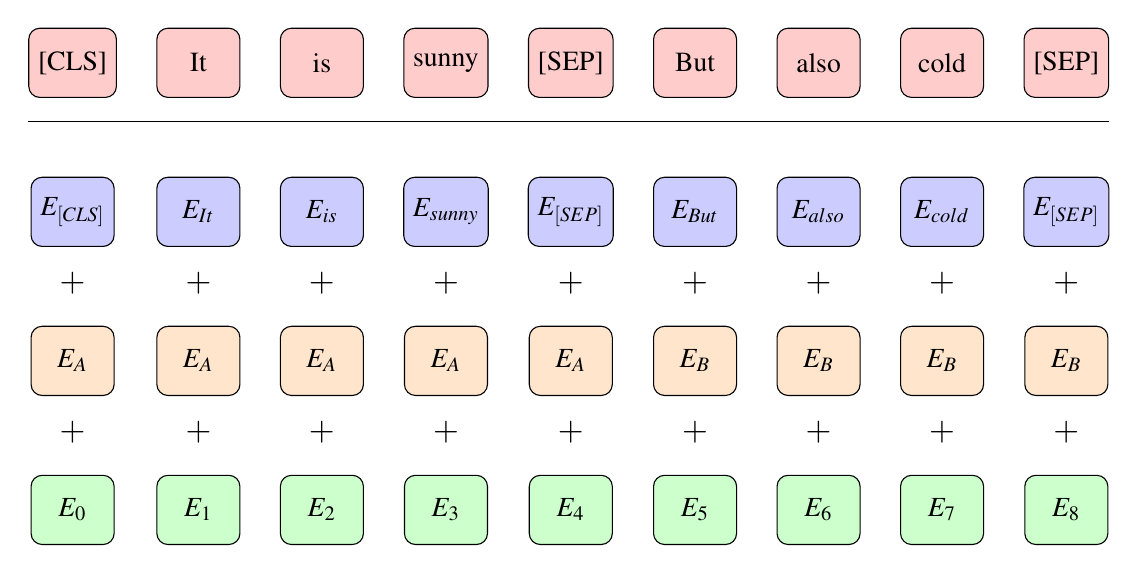
\begin{tikzpicture}[
  input/.style={rectangle, rounded corners, minimum height=2.5em, minimum width=3em, draw, fill=red!20},
  token/.style={rectangle, rounded corners, minimum height=2.5em, minimum width=3em, draw, fill=blue!20},
  seg_embed/.style={rectangle, rounded corners, minimum height=2.5em, minimum width=3em, draw, fill=orange!20},
  pos_embed/.style={rectangle, rounded corners, minimum height=2.5em, minimum width=3em, draw, fill=green!20},
  input_embed/.style={rectangle, rounded corners, minimum height=2.5em, minimum width=3em, draw, fill=purple!20},
  plus/.style={}
]

    % Tokens
    \node[input] (i1) {[CLS]};
    \node[input, right=0.5cm of i1] (i2) {It};
    \node[input, right=0.5cm of i2] (i3) {is};
    \node[input, right=0.5cm of i3] (i4) {sunny};
    \node[input, right=0.5cm of i4] (i5) {[SEP]};
    \node[input, right=0.5cm of i5] (i6) {But};
    \node[input, right=0.5cm of i6] (i7) {also};
    \node[input, right=0.5cm of i7] (i8) {cold};
    \node[input, right=0.5cm of i8] (i9) {[SEP]};

        % Tokens
    \node[token, below=1cm of i1] (t1) {$E_{[CLS]}$};
    \node[token, below=1cm of i2] (t2) {$E_{It}$};
    \node[token, below=1cm of i3] (t3) {$E_{is}$};
    \node[token, below=1cm of i4] (t4) {$E_{sunny}$};
    \node[token, below=1cm of i5] (t5) {$E_{[SEP]}$};
    \node[token, below=1cm of i6] (t6) {$E_{But}$};
    \node[token, below=1cm of i7] (t7) {$E_{also}$};
    \node[token, below=1cm of i8] (t8) {$E_{cold}$};
    \node[token, below=1cm of i9] (t9) {$E_{[SEP]}$};

    % Add plus nodes between inputs
    \draw ($(i1.south west) + (0,-0.3)$) -- ($(i9.south east) + (0,-0.3)$);

        % Segmentation embeddings
    \node[seg_embed, below=1cm of t1] (s1) {$E_{A}$};
    \node[seg_embed, below=1cm of t2] (s2) {$E_{A}$};
    \node[seg_embed, below=1cm of t3] (s3) {$E_{A}$};
    \node[seg_embed, below=1cm of t4] (s4) {$E_{A}$};
    \node[seg_embed, below=1cm of t5] (s5) {$E_{A}$};
    \node[seg_embed, below=1cm of t6] (s6) {$E_{B}$};
    \node[seg_embed, below=1cm of t7] (s7) {$E_{B}$};
    \node[seg_embed, below=1cm of t8] (s8) {$E_{B}$};
    \node[seg_embed, below=1cm of t9] (s9) {$E_{B}$};

    % Position embeddings
    \node[pos_embed, below=1cm of s1] (p1) {$E_{0}$};
    \node[pos_embed, below=1cm of s2] (p2) {$E_{1}$};
    \node[pos_embed, below=1cm of s3] (p3) {$E_{2}$};
    \node[pos_embed, below=1cm of s4] (p4) {$E_{3}$};
    \node[pos_embed, below=1cm of s5] (p5) {$E_{4}$};
    \node[pos_embed, below=1cm of s6] (p6) {$E_{5}$};
    \node[pos_embed, below=1cm of s7] (p7) {$E_{6}$};
    \node[pos_embed, below=1cm of s8] (p8) {$E_{7}$};
    \node[pos_embed, below=1cm of s9] (p9) {$E_{8}$};

    % Pluses at 0.25 between each (s, t) pair
    \node[above=0.25cm of $(s1)!.25!(t1)$, font=\large] {$+$};
    \node[above=0.25cm of $(s2)!.25!(t2)$, font=\large] {$+$};
    \node[above=0.25cm of $(s3)!.25!(t3)$, font=\large] {$+$};
    \node[above=0.25cm of $(s4)!.25!(t4)$, font=\large] {$+$};
    \node[above=0.25cm of $(s5)!.25!(t5)$, font=\large] {$+$};
    \node[above=0.25cm of $(s6)!.25!(t6)$, font=\large] {$+$};
    \node[above=0.25cm of $(s7)!.25!(t7)$, font=\large] {$+$};
    \node[above=0.25cm of $(s8)!.25!(t8)$, font=\large] {$+$};
    \node[above=0.25cm of $(s9)!.25!(t9)$, font=\large] {$+$};


    % Pluses at 0.25 between each (p, s) pair
    \node[above=0.25cm of $(p1)!.25!(s1)$, font=\large] {$+$};
    \node[above=0.25cm of $(p2)!.25!(s2)$, font=\large] {$+$};
    \node[above=0.25cm of $(p3)!.25!(s3)$, font=\large] {$+$};
    \node[above=0.25cm of $(p4)!.25!(s4)$, font=\large] {$+$};
    \node[above=0.25cm of $(p5)!.25!(s5)$, font=\large] {$+$};
    \node[above=0.25cm of $(p6)!.25!(s6)$, font=\large] {$+$};
    \node[above=0.25cm of $(p7)!.25!(s7)$, font=\large] {$+$};
    \node[above=0.25cm of $(p8)!.25!(s8)$, font=\large] {$+$};
    \node[above=0.25cm of $(p9)!.25!(s9)$, font=\large] {$+$};

\end{tikzpicture}
    \caption{BERT: Input Embeddings}
    \label{fig:bert_input}
\end{figure}

\subsection{Text Summarisation}\label{subsec:text-summarisation}
Text summarisation is the task of transforming a piece of text into a shorter  version that retains the most important information.
There are two overarching categories: extractive and abstractive text summarisation.
The former formulates the problem as a subset selection problem by returning only the most salient text excerpts from the original document (\cite{zhong-etal-2020-extractive}), while the latter aims to generate content anew, similar to how humans would do.

We will outline some key models that inspired our work below:
\begin{itemize}
    \item \textbf{Gokhan}: The authors employ an unsupervised summariser based on K-Means clustering of sentences encoded with SentenceBERT (\cite{reimers2019sentence}).
    However, their embeddings are pre-trained on general text, and they suggest that employing in-domain language models would result in a better performance.

    \item \textbf{AMUSE} (\cite{litvak-vanetik-2021-summarization}): The authors design an ETS system comprised of the following steps \begin{enumerate*}
        \item shortening of report with an existing Genetic Algorithm~\cite{litvak-last-2013-multilingual},
        \item encoding sentences with BERT vectors, and
        \item performing binary classification with LSTMs for salient sentence extraction
    \end{enumerate*}.
    They suggest that further work should incorporate \begin{enumerate*}
        \item efficient preliminary sentence removal, and
        \item additional neural modelling stages for the representation and detection of relevant input text parts.
    \end{enumerate*}

    \item \textbf{Hybrid model with RL} (\cite{zmandar-etal-2021-joint}): The authors train a joint extractive-abstractive summarisation model with reinforcement learning optimised for the ROUGE-2 F1 metric.
    Their networks are based on attentive LSTMs augmented with an additional copy mechanism (\cite{vinyals2015pointer}) achieving the second highest F1 score in the FNS21 competition.

    \item \textbf{T5} Hybrid (\cite{orzhenovskii-2021-t5}): The author used T5 (\cite{rayson2019t5}) for a hybrid model fine-tuned to generate the beginning of an abstractive summary and find the closest match of the output in the report’s full text.
    This is the best performing algorithm in the FNS21 competition but also the first to consider transformer models from an abstractive summarisation perspective in the FNP workshops so far.

\end{itemize}

In this work we will be solely exploring the extractive method, and more specifically - the \emph{supervised neural-based} (i.e., RNN, Transformer) type and the \emph{unsupervised graph-based} (i.e., TextRank, LexRank) type.


\subsection{LexRank}\label{subsec:lexrank}
LexRank (\cite{Erkan2004LexRankGC}) is an unsupervised extractive summarisation method consistently used as a baseline in the FNS21 and previous challenges.
It retrieves the most salient document sentences by computing their importance based on \emph{eigenvector centrality}.
To do that the algorithm creates a graph where each sentence represents a node and each edge is a weight between two nodes (\cite{Shearing2020AutomatedTS}).
The sentences are encoded as bag-of-words vectors of size $N$ - the vocabulary size, and the weight metric is a combination of tf-idf (Eq.\ref{eq:idf},\ref{eq:tfidf}) and cosine similarity - Eq.\ref{eq:cosinesimtfidf}.

\begin{equation}
    \text{idf}(t, D) = \log \frac{|D|}{|\{d \in D : t \in d\}|} \label{eq:idf}
\end{equation}

\begin{equation}
    \text{tf-idf}(t, d, D) = \text{tf}(t, d) \cdot \text{idf}(t, D)
    \label{eq:tfidf}
\end{equation}

\begin{equation}
    \text{tf\_idf\_cosine\_similarity}(s_1, s_2) = \frac{\sum_{t \in T} \text{tf-idf}(t, s_1, D) \cdot \text{tf-idf}(t, s_2, D)}{ \sqrt{\sum_{t \in T} \text{tf-idf}(t, s_1, D)^2} \cdot \sqrt{\sum_{t \in T} \text{tf-idf}(t, s_2, D)^2}}
    \label{eq:cosinesimtfidf}
\end{equation}

where $t$ is a term, $d$ is a document within a collection of documents/sentences $D$.

Also, $s_1$ and $s_2$ are two sentences and $T$ represents the set of all terms in both of them while $tf(t, d)$ denotes the term frequency of $t$ in $d$, and $idf(t, D)$ is the inverse document frequency of $t$ in the collection $D$.

The authors further propose finding the most important sentences by \begin{enumerate*}
    \item applying a threshold for the creation of edges with Eq.\ref{eq:cosinesimtfidf},
    \item building an adjacency matrix and normalizing it to produce \emph{transition probabilities},
    \item computing in an iterative fashion the \emph{eigenvector centrality} until convergence, and finally
    \item ranking sentences based on their \emph{lexical} PageRank (\cite{page1998anatomy}) score.
\end{enumerate*}
\section{Methodology}\label{sec:methodology}

\subsection{Data}\label{subsec:data}
The data for the FNS22 task is a collection of narrative parts of annual reports, converted from PDF to plain text.
As discussed in Section~\ref{subsec:fns} due to the rich visual representations in the PDFs, the resulting text suffers from various problems like
\begin{enumerate*}
    \item \emph{spacing inconsistencies} - mixing of tab-space word delimiters, over-segmentation (i.e., a split into incoherent chunks) and under-segmentation (i.e., merging of unrelated words),
    \item \emph{symbol encoding issues} - introduction of unreadable non-alphanumeric characters, and
    \item \emph{formatting issues} - words having different casing, hyphenation at the end of a line, etc
    \item \emph{conversion of tables to text} - financial figures spanning over multiple lines and being mixed with the text.
\end{enumerate*} (Figure~\ref{fig:pdf_to_text}).

% PDF-to-text conversion issues
\begin{figure}[ht]
    \centering
    \begin{enumerate}
        \item \begin{verbatim}
         Following my appointment as Chief
        E x e c u t i v e	in	J u l y	2 0 1 0 ,	g r e ate r	e m p h a s i s
        h a s	b e e n	p l a c e d	o n	f u l fi l l in g	t h e	s u p p l y	o f
        tonnage due under legacy contracts and
    \end{verbatim}
    \item \begin{verbatim}
        However,   the   Directors   further   believe   that   additional
        capital   	could   	be	  deployed	  to 	beneficial   	effect.
    \end{verbatim}
    \item \begin{verbatim}
        Opening net book amount 116,635 35,624 166,754 319,013
        Additions 51,380 7,647 307,546 366,573
    \end{verbatim}
    \item \begin{verbatim}
          This means that buyers can
        _0_@uk_ar06_front.indd   5 20/04/2007   09:13:30 05
        @UK PLC
        Annual Report and Accounts 2006
        use our network to purchase from their suppliers.
    \end{verbatim}
    \end{enumerate}
    \caption{PDF-to-text conversion issues.}
    \label{fig:pdf_to_text}
\end{figure}

To address these issues, we have developed a rigorous data cleaning pipeline that achieves the following key objectives:
\begin{enumerate*}
    \item handles space-tab mixing via hand-crafted rules (derived from observation\footnote{
      E.g., for some of the lines, characters were separated by spaces and words with tabs, hence the need for a custom rule.
    }),
    \item retains alphanumeric characters, punctuation, spaces, financial symbols, and
    \item removes sentences shorter than 3 words
\end{enumerate*}.

As discussed in Section~\ref{subsec:fns}, the annual reports are extremely long documents with an average length reported at 80 pages~\cite{litvak-vanetik-2021-summarization}.
Each one has at least two--three gold summaries provided by the FNS22 organisers, and we compute some statistics
\begin{enumerate*}
    \item helpful for grasping the nature of the output text, but also
    \item useful for the evaluation of the summarisation models
\end{enumerate*}.
On one hand, we can see that the average number of words in the longest summary is over $2,000$ (Figure~\ref{fig:longest_summary_word_count}), while the FNS22 regulations specify an expected output of at most $1,000$ words.
Furthermore, as we are not competing in the FNS22 task, for simplicity, during evaluation we will generate only summaries with at most 40 sentences.
We arrive at this number by observing that the median number of words in the longest summaries is 25 (Figure~\ref{fig:sentence_word_count}), and calculating that $\frac{1,000\text{words}}{25\text{words}}=40$ sentences can suffice.

\begin{figure}[ht]
    \begin{subfigure}{0.49\textwidth}
        \centering        \includegraphics[width=1\columnwidth]{../charts/longest_summary_word_count}
        \caption{Number of words in longest report summary}
        \label{fig:longest_summary_word_count}
    \end{subfigure}%
    \hfill
    \begin{subfigure}{0.49\textwidth}
        \centering
        \includegraphics[width=1\columnwidth]{../charts/sentence_word_count}
        \caption{Number of words in training sentences}
        \label{fig:sentence_word_count}
    \end{subfigure}
    \caption{Distribution of number of words in training sentences and report summaries}
    \label{fig:word_count}
\end{figure}

As we were only provided with the training and the validation FNS22 datasets (Table~\ref{tab:fns22-data}),
we decided to treat the validation set as a testing set (Table~\ref{tab:fns22-my-data})\footnote{
    We observed that two of the annual report files were empty, hence the difference of 3,361 and 3,363 (Table~\ref{tab:fns22-data} without testing set).
} and perform our own training-validation data split on a sentence level instead due to the significant variation in report lengths~\cite{litvak-vanetik-2021-summarization}.
\begin{table}[h]
    \centering
    \begin{tabular}{lrr r}
        \hline
        Data Type & Training + Validation & Testing & Total \\
        \midrule
        Report full text & 2,998 & 363 & 3,361 \\
        \bottomrule
    \end{tabular}
    \caption{Training-Validation-Testing Data Split}
    \label{tab:fns22-my-data}
\end{table}
Specifically, we use a 90--10 \emph{stratified split} (i.e., the label distribution is retained in both sets) for training and validation, respectively.
We are aware that a validation and a training sentence can come from the same report, but we claim that this is not problematic for the following reasons:
\begin{enumerate}
    \item Sentences are \emph{de-contextualised} (i.e., without references or dependencies to others, taken out of context) and \emph{shuffled}.
    \item Sentences contain a \emph{great deal of textual noise} due to the PDF-to-text conversion.
    \item Annual reports are \emph{numerous} but also \emph{extremely long} (i.e., containing a lot of sentences).
\end{enumerate}
Therefore, we believe that the training and validation sentences are to a large extent independent, and as for the process of sentence extraction, we refer you to Section~\ref{subsec:sentence_extraction} for an in-depth discussion.

\subsection{Sentence Extraction}\label{subsec:sentence_extraction}
We approach the annual report summarisation problem from a supervised perspective - we cast the task of Extractive Text Summarisation (ETS) as a binary classification problem defined on the sentence level.
More formally, we can describe the annual report as $d=\{s_{1}, s_{2}, \dots, s_{n}\}$, where $d$ is a document, represented in terms of sentences $s_{i}, \  1 \leq i \leq n$~\cite{liu2019finetuningbert}.

Then, a candidate summary\footnote{
    A candidate summary is generated from a model $m_{i}$ but it is not yet a \emph{best summary}.
} can be $c=\{s_{1}, s_{2}, \dots, s_{k} | s_{i} \in d \}, \ 0 \leq k \leq n$.
We further need to define the \emph{gold summary}, $c^{*}$ for a document $d$.
In the case of the FNS22 task, there are at least two summaries per report, hence we will use the following notation for the set of all gold summaries for each document $C^{*} = \{c^{*}_{1}, c^{*}_{2}, \dots, c^{*}_{p}\}$.
Furthermore, the supervised learning labels are $y_{i} \in \{1,0\}$ for each sentence $s_{i}$ in $d$ if the sentence is or is not in \textbf{\emph{any}} of the gold summaries $c^{*}_{j}$ for that document.
We argue that in order to increase the positive samples (i.e., the summarizing sentences) we should not restrict
ourselves to just one gold summary in the training process unlike~\cite{orzhenovskii-2021-t5}.
Our goal is to achieve better latent feature extraction of summaries through the employment of all existing data, hence using \textbf{\emph{any}} gold summaries.
However, we are aware that this approach is more likely to encounter standard ETS issues, specifically - extracted summary sentences could be retrieved from unrelated paragraphs in the report.
This can cause the \enquote{dangling anaphora} phenomenon, i.e.\ de-contextualised extracts are stitched together and can mislead the reader due to out-of-context references~\cite{lin2009summarization}.

While some authors~\cite{zmandar-etal-2021-joint} follow the greedy ROUGE-maximisation method of matching summary
sentences to document sentences (established in~\cite{nallapati2017summarunner}), we approach the problem in a
more practical and faster fashion.
After manual observation of the reports against their gold summaries, it became clear that almost for all sentences
belonging to $c^{*}_{i}$, there was an exact match with a sentence in the whole annual report $d$.

This hypothesis was proven correct by one of the FNS contestants~\cite{orzhenovskii-2021-t5} who reported that
99.4\% of the summaries were included in the report as whole subsequences.
Hence, after having pre-processed the text documents we iteratively match the sentences and generate the binary
classification labels ($\{1,0\}$ representing \emph{summary} and \emph{non-summary}, respectively) for both
the training and testing datasets.

We perform the sentence extraction as discussed above to produce a dataset (training and validation combined) of $3,554,800$ and $361,703$ sentences for classes 0 and 1, respectively.
Additionally, the training and validation sets are split in a 90--10 stratified fashion.

\subsection{Under-sampling and Data Augmentation}\label{subsec:data_augmentation}
Due to the fact that the annual reports are extremely long while the summaries are very short, the sentence dataset is highly imbalanced with a ratio of around 1:10.
Therefore, we took two\footnote{
    We also tried a third approach that is to augment sentences with the help of DINO~\cite{schick2021generating} used for high-quality
    semantic augmentation, but we did not manage to recreate the desired output.
} different approaches to balance the classes:
\begin{enumerate}
    \item \textbf{Random under-sampling} -- As described in~\cite{weiss2013foundations, wongvorachan2023undersampling}, we \emph{randomly remove 90\% of the sentences} from the majority class (i.e., non-summary sentences) to produce a ratio of 1:1 summary to non-summary sentences (Figure~\ref{tab:random_under_sampling}).
    \begin{table}[ht]
        \centering
        \begin{tabular}{lccc}
            \toprule
                & \textbf{initial data} & \textbf{90\% under-sampled training} & \textbf{validation} \\
            \midrule
                \textbf{label 0} & 3,199,319 & 319,931 & 355,481 \\
                \textbf{label 1} & 325,533 & 325,533 & 36,170 \\
            \bottomrule
        \end{tabular}
        \caption{90\% Random Under-sampling}\label{tab:random_under_sampling}
    \end{table}
    \item \textbf{Data Augmentation} -- We use the \emph{back-translation} technique~\cite{hoang-etal-2018-iterative} to generate new sentences from the minority class (i.e., summary sentences), followed by a 80\% random under-sampling of the majority class (Figure~\ref{tab:data_augmentation}).
    For that purpose, we translate all training summary sentences from English to French and back to English with the help of the MarianMT model~\cite{junczysdowmunt2018marian}\footnote{\url{https://huggingface.co/Helsinki-NLP/opus-mt-fr-en}}.
    The resulting dataset is then directly injected during the training process.
    Refer to Section~\ref{subsec:hyperparameters} for the experiments with the different data balancing techniques.
    \begin{table}[ht]
        \centering
        \begin{tabular}{lcccc}
        \toprule
            & \textbf{initial data} & \textbf{80\% under-sampled training} & \textbf{augmented training} & \textbf{validation} \\
        \midrule
            \textbf{label 0} & 3,199,319 & 639,863 & 639,863 & 355,481 \\
            \textbf{label 1} & 325,533 & 325,533 & 651,066 & 36,170 \\
        \end{tabular}
        \caption{Data Augmentation + 80\% Random Under-sampling}\label{tab:data_augmentation}
    \end{table}
\end{enumerate}

\newpage

\subsection{Recurrent Extractor Model}\label{subsec:rnn_model}
As our main recurrent model we propose a GRU-based architecture~\cite{cho-etal-2014-learning}, inspired by~\cite{zmandar-etal-2021-joint} and depicted in Figure~\ref{fig:rnn_model}. \\

\begin{minipage}[ht]{0.45\textwidth}
    The model consists of a word embedding layer, a fully-connected feed-forward neural network (FCFFNN), two bidirectional gated recurrent units (GRU) layers, a dot-product attention layer, and a linear projection layer with softmax activation.

    The word embedding layer is used to convert the pre-processed input sentence into a vector representation.
    One of our implementation innovations is that we use FinText's FastText word embeddings~\cite{rahimikia2021realised} because they
    \begin{enumerate*}
        \item are character-based and thus can handle noisy or out-of-vocabulary words, and
        \item are pre-trained on large corpora of financial news, achieving considerable in-domain performance improvements over general-purpose embeddings
    \end{enumerate*}.

    We use the FCFFNN layer to \emph{map the vectorized sentences to a higher-level representation} (similar to~\cite{saikh2020deep}) capturing more complex features or patterns from the input text, but also to \emph{reduce the dimensionality} of the input.

    Two stacked GRU layers are used to \emph{extract the latent recurrent features} from the compressed vector representation in both directions - forward and backward (refer to Section~\ref{subsec:rnn} for details).
\end{minipage}\hfill
\noindent\begin{minipage}[ht]{0.5\textwidth}
    \centering
    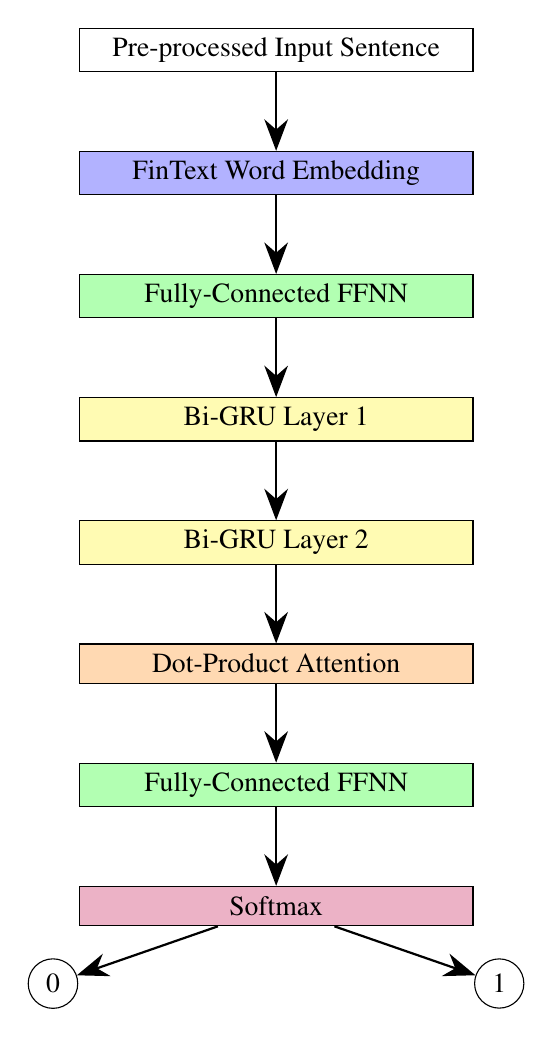
\begin{tikzpicture} [node distance = 0cm and 1cm,    box/.style={draw, rectangle, minimum height=0.5cm, minimum width=5cm},    arrow/.style={-{Stealth[length=4mm]}, thick, font=\footnotesize}]
        % Nodes
        \node[box] (input) {Pre-processed Input Sentence};
        \node[box, fill=blue!30, below=1cm of input] (we) {FinText Word Embedding};
        \node[box, fill=green!30, below=1cm of we] (fc) {Fully-Connected FFNN};
        \node[box, fill=yellow!30, below=1cm of fc] (biGRU1) {Bi-GRU Layer 1};
        \node[box, fill=yellow!30, below=1cm of biGRU1] (biGRU2) {Bi-GRU Layer 2};
        \node[box, fill=orange!30, below=1cm of biGRU2] (dpa) {Dot-Product Attention};
        \node[box, fill=green!30, below=1cm of dpa] (fc2) {Fully-Connected FFNN};
        \node[box, fill=purple!30, below=1cm of fc2] (sf) {Softmax};
        \node[circle, fill=white, draw=black, below left=0.5cm and 0.1cm of sf, minimum size=0.5cm] (bo1) {0};
        \node[circle, fill=white, draw=black, below right=0.5cm and 0.1cm of sf, minimum size=0.5cm] (bo2) {1};

        % Arrows
        \draw[arrow] (input) -- node[right] {} (we);
        \draw[arrow] (we) -- node[right] {} (fc);
        \draw[arrow] (fc) -- node[right] {} (biGRU1);
        \draw[arrow] (biGRU1) -- node[right] {} (biGRU2);
        \draw[arrow] (biGRU2) -- node[right] {} (dpa);
        \draw[arrow] (dpa) -- node[right] {} (fc2);
        \draw[arrow] (fc2) -- node[right] {} (sf);
        \draw[arrow] (sf) -- node[right] {} (bo1);
        \draw[arrow] (sf) -- node[right] {} (bo2);
    \end{tikzpicture}
    \captionof{figure}{GRU-based extractive model}
    \label{fig:rnn_model}
\end{minipage}

We further implement the scaled dot-product attention (Eq.\ref{eq:attention_score} from~\cite{vaswani2017attention}) to
compute a new weighted context-aware representation from the extracted features by the GRU layers.
The final layer is a fully-connected feed-forward neural network (FCFFNN) with a softmax activation function, which is
used to \emph{map the latent features to a binary classification} of the input sentence.

\subsection{Training}\label{subsec:training}
We trained both models on Tesla V100-SXM2-16GB\footnote{
    We extend our gratitude to the University of Manchester's Computational Shared Facility (CSF) for kindly agreeing to provide us with the computational resources for this research.
} and provide the following specifications:
\begin{enumerate}
    \item \textbf{RNN architectures} - below we provide the common general details, however for an in-depth discussion on the hyperparameter tuning, see Section~\ref{subsec:hyperparameters}.
        \begin{itemize}
            \item \textbf{Loss function:} Binary cross-entropy loss
            \item \textbf{Optimizer:} Adam~\cite{kingma2017adam}
            \item \textbf{Batch size:} 32
            \item \textbf{Epochs:} set to 60, but due to early stopping, the model practically trains for less than 10 epochs
            \item \textbf{Early stopping:} patience (i.e., the number of epochs to wait for improvement based on validation loss) set to 1
        \end{itemize}
    \item \textbf{FinBERT} - We followed the prescribed fine-tuning specifications provided in the original BERT paper~\cite{devlin-etal-2019-bert}:
        \begin{itemize}
            \item \textbf{Loss function:} Binary cross-entropy loss
            \item \textbf{Optimizer:} Adam~\cite{kingma2017adam}
            \item \textbf{Batch size:} 32
            \item \textbf{Epochs:} 3 - we found that the model started to over-fit after 3 epochs
            \item \textbf{Learning rate:} 2e-5
            \item \textbf{Weight decay:} 0.01
        \end{itemize}
\end{enumerate}


\subsection{RNN: Hyperparameter Tuning}\label{subsec:hyperparameters}
We have experimented with a number of hyperparameters for our recurrent model, including the use of a FCFFNN,
the recurrence type, the hidden units, the effect of applying attention, the dropout rate, the learning rate, and the effect of data augmentation.

For the analysis we will be extensively using the test accuracy, $F1$-score, and the \emph{summary recall} metric.
The latter is defined as the ratio of the number of correctly predicted summary sentences to the total number of summary sentences in the test dataset.
We consider this metric to be extremely relevant because in the context of extractive summarisation, our goal is to minimise the Type II error (i.e., the number of sentences that should be in the summary but are not).
Our reasoning is that our classifier must be as good as possible in recognising salient sentences (i.e., summarising sentences) even if it introduces some false positives (i.e., non-summarising sentences).
In practice, the user can always remove irrelevant sentences, but it is much harder to add sentences that should have already been in the summary.

We would also like to remind the reader of the label distribution per dataset (Tables~\ref{tab:random_under_sampling} and~\ref{tab:data_augmentation}).
It is worth noting that although we have managed to balance the training set with the help of random under-sampling and data augmentation,
our validation and testing sets are left unchanged (i.e., they are imbalanced).

Each sentence in the report is represented as a (100, 300)--sized word embeddings vector, where 100 is the longest possible sentence length (i.e., implying long sentences are trimmed) and 300 is the dimensionality of the word embeddings.
We test the effect of inserting an FCFFNN layer between the word embeddings and the GRU layers (each with 64 hidden units) and arrive at the following results:
adding an FCFFNN layer increases Summary Recall by 2.5\% (Fig.~\ref{fig:summary_recall_FFNN_effect}), but marginally reduces Test Accuracy by less than 1\% (Fig.~\ref{fig:test_accuracy_FFNN_effect}).
We attribute the increase in Summary Recall to the fact that the FCFFNN layer is able to extract an additional mix of features from the word embeddings, which are then used by the GRU layers to make better predictions.
As for the Test Accuracy, we believe that the small decrease is insignificant and we therefore choose to use the FCFFNN layer in our final model.

\begin{figure}[ht]
    \begin{subfigure}{0.49\textwidth}
        \centering \includegraphics[width=1\columnwidth]{../charts/summary_recall_FFNN_effect}
        \caption{Effect of FCFFNN layer on summary recall}
        \label{fig:summary_recall_FFNN_effect}
    \end{subfigure}%
    \hfill
    \begin{subfigure}{0.49\textwidth}
        \centering
        \includegraphics[width=1\columnwidth]{../charts/test_accuracy_FFNN_effect}
        \caption{Effect of FCFFNN layer on test accuracy}
        \label{fig:test_accuracy_FFNN_effect}
    \end{subfigure}
    \caption{Effect of FCFFNN layer on summary recall and test accuracy}
    \label{fig:FCFFNN}
\end{figure}

We also explore the effect of using back-translated data (Section~\ref{subsec:data_augmentation}) on the model performance.
Results shown in Fig.~\ref{fig:data_augmentation_effect} suggest that the data augmentation does not improve the $F1$-score or the summary recall with a statistically significant margin.
At the same time, it seems to be amplifying the effect of the scaled dot-product attention (Section~\ref{subsec:seq2seq}, Figure~\ref{fig:summary_recall_data_augmentation_effect}).
\begin{figure}[ht]
    \begin{subfigure}{0.49\textwidth}
        \centering \includegraphics[width=1\columnwidth]{../charts/Summary Recall comparison}
        \caption{Effect of data augmentation on summary recall}
        \label{fig:summary_recall_data_augmentation_effect}
    \end{subfigure}%
    \hfill
    \begin{subfigure}{0.49\textwidth}
        \centering
        \includegraphics[width=1\columnwidth]{../charts/f1 score comparison}
        \caption{Effect of data augmentation on $F1$-score}
        \label{fig:f1_score_comparison_data_augmentation_effect}
    \end{subfigure}
    \caption{Effect of back-translation data augmentation on summary recall and $F1$-score}
    \label{fig:data_augmentation_effect}
\end{figure}
While we are disappointed by these results, we believe that there can be a number of reasons for this.
For a machine translated sentence $s^m_i$ and its original sentence $s_i$, we \hypertarget{data_augment_hypothesis}{\emph{hypothesise}} that:
\begin{enumerate*}
    \item $s^m_i$ contain a similar amount of noise as $s_i$ (due to the pdf-to-text conversion process),
    \item $s^m_i$ does not introduce enough variation to $s_i$ (i.e., $s^m_i$ and $s_i$ are too similar), and
    \item while financial language itself is very domain-specific, it is not very semantically diverse (i.e., metaphors, idioms, etc. are limited in use)
\end{enumerate*}.

% GRU vs LSTM + hidden size 64 vs 256
In our proposed architecture we choose a bidirectional GRU (Bi-GRU) instead of a Bi-LSTM because
\begin{enumerate*}
    \item GRUs have a simpler structure than LSTMs and are easier to train (Section~\ref{subsec:rnn}), and
    \item our experiments show that GRUs outperform LSTMs with 1\% in terms of Summary Recall
\end{enumerate*}.
Furthermore, in terms of the hidden units, we select 64 over 256 because:
\begin{enumerate*}
    \item the architecture has $143,938$ and $2,050,306$ parameters, respectively (i.e., $256$ would result in an over-parameterised model),
    \item almost 4\% increase in Summary Recall (Fig.~\ref{fig:64vs256_summary_recall}),
    although a 2\% decrease in Test Accuracy (Fig.~\ref{fig:test_accuracy_dropout_and_hidden_size}), if we use $64$ hidden units.
\end{enumerate*}
\begin{figure}[ht]
    \begin{subfigure}{0.49\textwidth}
        \centering \includegraphics[width=1\columnwidth]{../charts/64vs256_summary_recall}
        \caption{Summary Recall: 256 vs 64 hidden units + dropout}
        \label{fig:64vs256_summary_recall}
    \end{subfigure}%
    \hfill
    \begin{subfigure}{0.49\textwidth}
        \centering
        \includegraphics[width=1\columnwidth]{../charts/test_accuracy_dropout_and_hidden_size}
        \caption{Test Accuracy: 256 vs 64 hidden units + dropout}
        \label{fig:test_accuracy_dropout_and_hidden_size}
    \end{subfigure}
    \caption{Effect of hidden units and dropout on summary recall and test accuracy}
    \label{fig:dropout_and_hidden_size}
\end{figure}

From the above experiments it is hard to make any certain conclusions on the effect of dropout\footnote{
    It would make more sense for its application in the over-parameterised model, though this does not seem to be the case (Fig.~\ref{fig:dropout_and_hidden_size}).
} or the use of an attention mechanism (Section~\ref{subsec:seq2seq}).
We believe that only one \emph{single-head attention} is not sufficient to learn all the complex relationships between words in the sentences.
Our reasoning is that because a particular head specializes to only specific language aspects (i.e., syntactic, semantic, etc)~\cite{clark-etal-2019-bert}),
for future experiments it would be much more reasonable to use multiple heads instead.
Nevertheless, there still are some practical benefits of attention to our extractive summarisation system which we will discuss in Section~\ref{sec:evaluation}.

Overall, four variations of the RNN model engage our focus based on the results above and our design decisions (Figure~\ref{fig:summary_recall_data_augmentation_effect}):
\begin{enumerate}
    \item GRU-base with 90\% under--sampling
    \item GRU-base with 90\% under--sampling + attention
    \item GRU-base with 80\% under--sampling + data augmentation
    \item GRU-base with 80\% under--sampling + data augmentation + attention
\end{enumerate}
Because our binary classification metrics do not demonstrate any significant differences between them, we will
test their performance with ROUGE during the evaluation phase (Section~\ref{sec:evaluation}).
\chapter{Evaluation}\label{ch:evaluation}
In this chapter we outline the evaluation process of our models.
For that purpose, we describe how we use the ROUGE metrics (Section~\ref{subsec:rouge}) to compute the
similarity between the gold and candidate summaries, and how we arrive at the final evaluation aggregation (Section~\ref{sec:evaluation-mechanism}).
Afterwards, we provide the results of our evaluation (Section~\ref{sec:quantitative-evaluation}), where we compare our models to the baselines and official FNS models.
Finally, we discuss the qualitative limitations of our produced summaries (Section~\ref{sec:qualitative-discussion}) before we conclude our work in Chapter~\ref{ch:conclusion}.

\section{Evaluation Mechanism}\label{sec:evaluation-mechanism}
To assemble a candidate summary $c_{i}$ we prepare the sentences $s_{j}^{i}$ from a report $d_{m}$ (e.g., embed or tokenize sentences for the GRUs and FinBERT, respectively).
Afterwards, we feed them into our model computing the output summary probabilities $p_{j}^{i}$, and then we select the
top-$k$ sentences ($k=40$, Section~\ref{sec:data}) based on the highest sentence probabilities $p_{j}^{i}$.
Finally, we concatenate them to form the summary $c_{i}$ in natural order (i.e., the order in the input text),
but also trim it to the maximum length of $1,000$ words (Section~\ref{sec:fns}).

In general, to assess the quality of a candidate summary $c$, we measure its similarity with the gold summary $c^{*}$
based on their n-gram overlap $R=(c, c^{*})$, where $R$ is the ROUGE-2\footnote{
        We use a slightly different but faster version of ROUGE compared to the official metric~\cite{lin2004rouge}.
        It can be accessed at: \url{https://github.com/pltrdy/rouge}. \\
        The FNS evaluation metric is the $F1$-score of ROUGE-2, and we will use it for the final evaluation.
} metric(\cite{lin2004rouge}).
For the FNS task due to the extractive nature of our approach we will evaluate our models based on
the ROUGE-L-maximising\footnote{
    We say ROUGE-L-maximising for conciseness, because ROUGE is a metric with precision and recall components, which are combined into a single $F1$ score.
    It is precisely the $F1$ score that we maximise.
    However, we are aware this introduces more complexity to our naming convention, hence we will use the term ROUGE-L-maximising.
} $c^{*\max}_{i}$ gold summary (Section~\ref{subsec:rouge}), i.e.,

\begin{equation}\label{eq:rouge_max}
    c^{*\max} = \underset{c^{*} \in C^{*}}{\operatorname{argmax}} \text{ROUGE-L}(c, c^{*}_{i})
\end{equation}
where $C^{*}$ is the set of gold summaries for a given report $d$, and $c^{*\max}_{i}$ is the gold summary with maximal ROUGE-L score with the candidate summary $c$.

The intuition is that by extracting multiple sentences from the report, our generated candidate summary can
retain sentences from \emph{any} of the gold summaries.
Hence, there must be at least one such gold summary where the longest common subsequence overlap (ROUGE-L) is maximal.
The practical implications are that two models, $m_{1}$ and $m_{2}$ can produce two different candidate summaries
$c_{1}$ and $c_{2}$, respectively.
Their individual evaluation is based on gold summaries $c^{*}_{1}$ and $c^{*}_{2}$ (which can be the same when the
candidates $c_{1}$ and $c_{2}$ are identical).
This guarantees that we are always comparing candidate summaries based on their maximal evaluation scores (i.e., their maximal summarising potential).

Therefore, the final evaluation score for a model $m$ is the average ROUGE-2 score\footnote{
    Here, once again we mean the $F1$-measure of ROUGE-2.
} between the candidate summaries $c_{i}$ and their corresponding \emph{ROUGE-L-maximising gold summaries} $c^{*\max}_{i}$, i.e.,
\begin{equation}\label{eq:rouge_final}
    r_{m} = \frac{1}{|C|} \sum_{i=1}^{|C|} \text{ROUGE-2}(c_{i}, c^{*\max}_{i})
\end{equation}
where $|C|$ is the number of candidate summaries $c_{i}$.

\section{Quantitative Evaluation}\label{sec:quantitative-evaluation}
Following this evaluation mechanism, we compare our models in terms of their ROUGE metrics in Table~\ref{tab:rouge_performance_validation}, which
shows the results on the official validation set used as a testing set for our models.
We again wish to remind the reader that we were not provided with the FNS22 testing set (Section~\ref{sec:data}).

Therefore, in our comparison we include the following FNS22 models, namely:
\begin{enumerate}
    \item team LIPI's T5 model~\cite{el-haj-etal-2022-financial} (testing data is only available), which is the completely based on the T5-LONG-EXTRACT and also the best English model in that edition;
    \item team LSIR's mT5 model~\cite{foroutan-etal-2022-multilingual}, which is the best model overall for all languages in the competition (multilingual for English, Spanish, and Greek);
    \item the Longformer-Encoder-Decoder (LED)~\cite{khanna-etal-2022-transformer}
    \item the Top-K Narrative Extractor (NE) ~\cite{shukla-etal-2022-dimsum}  ranking in the top three models overall for Spanish and Greek;
\end{enumerate}
We have the official English validation results for all but the LIPI's T5, for which we are going to use their testing evaluations (we are aware that this comparison is somewhat unfair).
We will highlight the FNS models with a $\heartsuit$, and our top-performing ones with a $\spadesuit$ for ease of reference.

\begin{table}[ht]
    \centering
    \begin{tabular}{lccc}
        \toprule
        \textbf{Model} & \textbf{ROUGE-1} & \textbf{ROUGE-2} & \textbf{ROUGE-L} \\
        \midrule
            $\heartsuit$ Top-K NE & \textbf{0.546} & \textbf{0.425} & - \\
            $\spadesuit$ FinBERT-base & \emph{0.544} & \emph{0.382} & \emph{0.524} \\
            $\heartsuit$ LIPI's T5 (\emph{official testing set}) & 0.496 & 0.374 & 0.487 \\
            FinBERT-base + back-translation & 0.490 & 0.321 & 0.468 \\
            $\heartsuit$ LSIR's mT5 & 0.440 & 0.301 & 0.423 \\
            $\heartsuit$ LED & 0.442 & 0.302 & 0.434 \\
            $\spadesuit$ GRU-base + attention + back-translation & \emph{0.276} & \emph{0.106} & \emph{0.249} \\
            GRU-base + back-translation & 0.266 & 0.100 & 0.247 \\
            LexRank & 0.250 & 0.086 & 0.227 \\
            TaxtRank & 0.220 & 0.064 & 0.196 \\
            GRU-base & 0.220 & 0.063 & 0.201 \\
            GRU-base + attention & 0.221 & 0.062 & 0.204 \\
        \bottomrule
    \end{tabular}\caption{ROUGE $F1$ Scores on official validation set (used as testing in our models)}
    \label{tab:rouge_performance_validation}
\end{table}

We can provide the following commentary on the results:
\begin{itemize}
    \item Our best performing model, FinBERT-base~\cite{yang2020finbert}, which is a pre-trained on financial communication documents,
        achieves an average ROUGE-2 score of $0.382$, which outperforms by $0.081$ on the validation set the best performing
        model overall in the FNS22 competition - \emph{LSIR's mT5}~\cite{foroutan-etal-2022-multilingual}.
        Furthermore, our FinBERT-base also seems to \emph{slightly outperform the best English model in the FNS22} - LIPI's T5~\cite{el-haj-etal-2022-financial} with $0.008$,
        though this comparison is not entirely fair as we are not using the same datasets.
        Regarding the other FNS models, we observe that our FinBERT-base beats the LED~\cite{khanna-etal-2022-transformer} with a similar margin as the LSIR's mT5.
        However, the Top-K remains with the highest ROUGE-1 and ROUGE-2 $F1$ measures.
        Surprisingly, data augmentation does not improve the performance of our FinBERT-base, and we believe this was caused by
        the \hyperlink{data_augment_hypothesis}{back-translation hypothesis} we made in Section~\ref{sec:hyperparameters}, which can be leading to over-fitting.
        Nevertheless, both models clearly outperform the official baselines: LexRank~\cite{Erkan2004LexRankGC} and TextRank~\cite{mihalcea-tarau-2004-textrank}.
    \item The GRU-base + attention + back-translation model is the best performing model out of all recurrent neural architectures.
    While preliminary binary classification results did not show any considerable differences between the models, clearly
    \begin{enumerate*}[label=(\alph*)]
        \item the attention mechanism helps the model to better recognise the summarising sentences (i.e., attends to the most descriptive linguistic features), and
        \item the back-translation data augmentation significantly improves the practical performance of the model (i.e., the probability distribution of the summarising sentences),
              which is clearly not the case for our FinBERT model.
    \end{enumerate*}
    Additionally, we must note that except of the Top-K NE~\cite{shukla-etal-2022-dimsum}, all other FNS models are transformer-based,
    hence they have more complex architectures and attention mechanisms than our GRU-based models with single-head attention (Sections~\ref{sec:transformers} and~\ref{sec:rnn_model}).
    \item At the same time, we acknowledge that the universal summarisation baselines: LexRank and TextRank, outperform
        our simple GRU models (Table~\ref{tab:rouge_performance_validation}), and we attribute this to both:
    \begin{enumerate*}[label=(\alph*)]
        \item the lack of sufficient descriptive training data from the positive class (i.e., the summarising sentences, Table~\ref{tab:random_under_sampling}),
        \item the 90\% random under-sampling of the majority class data (see Section~\ref{sec:data}), and
        \item the summary generation process of selecting the top-$k$ sentences based on their sorted probabilities (see discussion in Sections~\ref{sec:qualitative-discussion} and~\ref{sec:limitations}).
    \end{enumerate*}
\end{itemize}

\newpage

\section{Qualitative Discussion}\label{sec:qualitative-discussion}
After having established the quantitative performance of our models, we now turn to the qualitative discussion of the results.
For a random annual report we generated a summary using the FinBERT-base + data augmentation model and
the GRU-base + attention model (see Figures~\ref{fig:finbert_summary},~\ref{fig:rnn_summary}).
where green colour indicates the summarising sentences, and red colour -- the non-summarising sentences).
We chose these models over the best ones because they have slightly lower ROUGE scores, and make more mistakes, which will help us identify the issues in the summarisation process.
We can make the following conclusions based on observation:
\begin{enumerate}
    \item The FinBERT model has \emph{around 50\% of its contents} belonging to any of the gold summaries (Figure~\ref{fig:finbert_summary}),
        while all other sentences look very convincing in terms of their summarising potential (i.e., they are informative of the financial situation but also concise)
    \item At the same time, the GRU-model has the opposite characteristics:
    \begin{enumerate*}[label=(\alph*)]
        \item none of its sentences are in the gold summary (Figure~\ref{fig:rnn_summary}), while
        \item all of them are very long, containing uninformative but diverse sets of words, which in turn results in higher ROUGE scores
    \end{enumerate*}.
    This clearly represents the problem of using ROUGE as a metric for summarisation since it is only measures the lexical overlap, while being semantically unaware~\cite{akter-etal-2022-revisiting}.
\end{enumerate}
While we acknowledge that the GRU model seems to be \emph{biased towards long and noisy sentences}, we must note that in the example
only $5$ sentences have been generated to fit the word limit.
Therefore, we believe the summary generation process (i.e., the mechanism to combine predicted sentences into a single summary) further
exacerbates the accuracy of the summarisation.

Although, the practical results from Figures~\ref{fig:rnn_summary} might seem disappointing, we must once again remind the reader that the reports are extremely
long with an average number of sentences and words at around $2,700$ and $58,000$, respectively~\cite{litvak-vanetik-2021-summarization}.
Meanwhile, we are constrained to producing a summary of at most $40$ sentences (Section~\ref{sec:data}) or $1,000$ words (Section~\ref{sec:fns}).

\newpage

\chapter{Conclusion}\label{ch:conclusion}
In this section we summarise the main contributions of our work, highlighting its innovational aspects and discussing its limitations.

\section{Summary of Achievements}\label{sec:summary}
In this project we have explored the problem of summarising UK annual reports.
To deal with the significant amount of noise in the plain text of these glossy documents, we have built a rigorous pre-processing pipeline (Section~\ref{sec:data}).
We have further implemented a sentence extraction phase where we generate binary labels ($1$ being summary, $0$ - non-summary) from the reports and their multiple gold summaries (Section~\ref{sec:sentence_extraction}).
Once our datasets are created, we
\begin{enumerate*}[label=(\alph*)]
    \item design a Recurrent Neural Network (RNN) architecture (Section~\ref{sec:rnn_model}), and
    \item fine-tune a financial Transformer model - FinBERT (Section~\ref{sec:finbert})
\end{enumerate*},
training them in a supervised manner for a binary classification task (Sections~\ref{sec:training} and~\ref{sec:hyperparameters}).
We quantitatively evaluate our models with the ROUGE metric and demonstrate them outperforming traditional baselines (Chapter~\ref{ch:evaluation}).
Furthermore, at least for FinBERT we observe a clear ROUGE-2 improvement on the validation set over the best overall FNS22 model~\cite{foroutan-etal-2022-multilingual}.
Additionally, we show that our FinBERT also achieves competitive performance with the best FNS22 English model,
although noting that the our models are tested on different data (Section~\ref{sec:data}).
We also discuss the quality of the produced summaries (Section~\ref{sec:qualitative-discussion}), and in
Section~\ref{sec:limitations} we describe in more depth the limitations of our system and possible solutions.
\\
In terms of \emph{innovational aspects} of our project in the context of the FNS challenge, we are the first to our knowledge that:
\begin{itemize}
    \item \emph{Integrate FinText word embeddings} - While some FNS21 competitors use general-domain sentence embeddings
    based on BERT~\cite{litvak-vanetik-2021-summarization, gokhan-etal-2021-extractive}, we represent sentences as
    a vector of word embeddings purpose-built for financial text analysis~\cite{rahimikia2021realised}.
    \item \emph{Perform back-translation as data augmentation} - In contrast to approaches where only the first 10\% of
    the annual report is used~\cite{orzhenovskii-2021-t5}, we over-sample the summarising sentences (minority class)
    by back-translating from French.
    \item~\emph{Fine-tune FinBERT~\cite{yang2020finbert} for extractive summarisation} - Transformer-based models have become increasingly
    popular in the FNP22 Workshop~\cite{khanna-etal-2022-transformer, pant-chopra-2022-multilingual},
    where some have used FinBERT for classifying definitions~\cite{ghosh-etal-2022-finrad},
    detecting hypernyms~\cite{peng-etal-2022-discovering}, and classifying financial sentiments~\cite{stepisnik-perdih-etal-2022-sentiment}.
    However, we are the first to adapt FinBERT for extractive summarisation.
\end{itemize}

\section{Discussion of Limitations}\label{sec:limitations}
Although, both our models have outperformed the baselines on ROUGE-2 and the fine-tuned FinBERT has achieved competitive
performance for the FNS22 task, there are several limitations that we would like to discuss:
\begin{itemize}
    \item \emph{Sentence embedding} - Although, we note our use of domain-specific FastText word embeddings due to their
    ability to handle noise and outperform general-domain embeddings~\cite{rahimikia2021realised}, we do not perform
    any sentence--level aggregation (i.e., dimensionality reduction) like averaging to condense the overall representation.
    While, this was a deliberate design decision to better capture the relationship between individual words,
    our sentence vectors became of size $(100, 300)$ instead of $(300,)$, which became more computationally expensive.
    Although, we are aware that FastText~\cite{bojanowski-etal-2017-enriching} provides average-pooling for any sequence,
    we were pessimistic of using it due to the loss of word order information (e.g., ``the company is good'' being represented just as ``is the company good'').
    Therefore, a limitation of our work is that we do not investigate the impact of using sentence embeddings
    (be it with positional encoding or average-pooling) on the performance of our models.
    \item \emph{Non-exhaustive evaluation} - Due to the FNS models being proprietary, and also evaluated on the official testing set,
    we are unable to make a more comprehensive comparison with the other models.
    However, in an ideal scenario we would perform further quantitative and qualitative evaluation of our performance.
    \item \emph{Summary Generation} - In our work we take top $k$ sentences based on the model's output probability distribution (Chapter~\ref{ch:evaluation}).
        However, this is a very simplistic approach to summarisation that
        \begin{enumerate*}[label=(\alph*)]
            \item introduces incoherence issues (like the \emph{dangling anaphora phenomenon} from Section~\ref{sec:sentence_extraction}),
            \item trims the last sentence to fit the $1,000$ word limit, and it
            \item does not account for the \emph{informativeness} of the individual sentences
        \end{enumerate*}.
        To address the incoherence issues, we can try resolving the coreferences in the either through a
        graph-based approach on the generated summary~\cite{sonawane2016coreference}, or by introducing a more complex
        encoder architecture that represents and attends to entities as well as sentences~\cite{Huang2021ExtractiveSC}.
        Regarding the trimming heuristic, a natural improvement can be to use text compression techniques for the final predicted sentence~\cite{ghalandari2022efficient, KNIGHT200291}.
        As for the third point, we believe this is very exacerbating reason why our GRU architecture returns a summary
        without any single whole--sentence overlap with the gold standard (Fig.~\ref{fig:rnn_summary}).
        Instead, what~\cite{zmandar-etal-2021-joint} propose is a reinforcement learning approach which incorporates
        the \emph{sentence-level} ROUGE-2 score with the whole gold summary.
        While this method is much more sophisticated, it conveys the intuitive idea that the top-$k$ sentences comprising the
        \emph{optimal candidate summary} should be \emph{greedily maximising the global summary-level ROUGE-2} score.
\end{itemize}

\section{Future Work}\label{sec:future-work}
While in our project we only consider the narrative summarisation of
financial reports already converted to plain text, we propose the following pipeline as a direction for future work:
\begin{enumerate}
    \item \emph{PDF-to-Text} - Integrate into the summarisation system a PDF-to-Text conversion tool for annual
    reports like the CFIE-FRSE\footnote{\url{https://github.com/drelhaj/CFIE-FRSE}}~\cite{elhaj2019multilingual}, which
    also extracts the text into 8 generic section headers (Section~\ref{sec:uk-annual-reports}).
    \item \emph{Text-to-Summary} - Implement an extractive method that addresses the limitations from Section~\ref{sec:limitations},
    or alternatively, an abstractive method producing \emph{lay summaries} for non-expert users~\cite{vinzelberg2023lay, Guo2020AutomatedLL}.
    \item \emph{Text-to-Analysis} - Apply NLP techniques like sentiment analysis~\cite{araci2019finbert}, named entity recognition
   ~\cite{zhang2022finbertmrc}, and detection of forward-looking sentences~\cite{stihec-etal-2021-preliminary},
    to extract useful information from the summary and the text.
    Additionally, important financial disclosure characteristics as amount, tone, and transparency~\cite{li2010textual, Li2011TextualAO}
    would be beneficial for AF researchers and users.
    \item \emph{Packaged Software} - Build a drag-and-drop software application that allows users to upload a PDF file of an
    annual report, where the backend will perform the steps above and return a summary.
    The suggested textual analysis features could be integrated as interactive visual elements.
    Furthermore, through recognising company names, the system could also provide dashboard of news and stock prices
    with the help of company-to-identifier mapping~\cite{el-haj2019retrieving}
    (i.e., getting the company ticker, e.g., \emph{NASDAQ: AAPL} for Apple Inc).
\end{enumerate}

%\printbibliography %Prints bibliography
\bibliography{refs}             % this causes the references to be
                                % listed

\bibliographystyle{alpha}       % this determines the style in which
                                % the references are printed, other
                                % possible values are plain and abbrv
%% Appendices start here
%\appendix
\chapter{Appendix}\label{ch:appendix}
\section{UK annual report example}\label{sec:uk-annual-report-example}
\begin{figure}[ht]
    \begin{subfigure}{0.49\textwidth}
        \centering
        \includegraphics[width=1\columnwidth]{../charts/1}
    \end{subfigure}%
    \hfill
    \begin{subfigure}{0.49\textwidth}
        \centering
        \includegraphics[width=1\columnwidth]{../charts/2}
    \end{subfigure}~\caption{Excerpts from Oxfam's 2021--2022 (glossy) annual report}
    \label{fig:oxfam1}
\end{figure}

\begin{figure}[ht]
    \begin{subfigure}{0.49\textwidth}
        \centering
        \includegraphics[width=1\columnwidth]{../charts/3}
    \end{subfigure}%
    \hfill
    \begin{subfigure}{0.49\textwidth}
        \centering
        \includegraphics[width=1\columnwidth]{../charts/4}
    \end{subfigure}~\caption{Excerpts from Oxfam's 2021--2022 (glossy) annual report}
    \label{fig:oxfam2}
\end{figure}

\vfill 

\section{Example Model Summaries}\label{sec:example-model-summaries}
\begin{figure}[ht]
    \centering
    \includegraphics[width=\textwidth]{../charts/transformer-example-summary}
    \caption{Example summary from the FinBERT-base + data augmentation model.}
    \label{fig:finbert_summary}
\end{figure}

\begin{figure}[ht]
        \centering
        \includegraphics[width=\textwidth]{../charts/rnn_summary}
        \caption{Example summary from the GRU-base + attention model.}
        \label{fig:rnn_summary}
\end{figure}

\end{document}
